\documentclass[11pt,a4paper]{article}
\usepackage[margin=2.2cm]{geometry}
\usepackage{graphicx}
\graphicspath{{../results/images/}}
\usepackage{booktabs}
\usepackage{tabularx}
\usepackage{array}
\usepackage{xcolor}
\usepackage{float}
\usepackage{caption}
\usepackage{hyperref}
\usepackage{fancyhdr}

\definecolor{okgreen}{RGB}{20,120,60}
\definecolor{warnorange}{RGB}{200,110,0}
\definecolor{badred}{RGB}{180,30,30}
\newcommand{\ok}{\textcolor{okgreen}{\textbf{OK}}}
\newcommand{\warn}{\textcolor{warnorange}{\textbf{Check}}}
\newcommand{\bad}{\textcolor{badred}{\textbf{Not usable}}}
\newcommand{\SW}{\textsuperscript{SW}}
\newcommand{\CALC}{\textsuperscript{C}}
\newcommand{\EST}{\textsuperscript{E}}

\pagestyle{fancy}
\fancyhf{}
\lhead{Sisyphus IoT Sensor Node}
\rhead{Flow Simulation Report}
\cfoot{\thepage}

\hypersetup{colorlinks=true,linkcolor=black,urlcolor=blue}
\setlength{\parskip}{4pt}
\setlength{\parindent}{0pt}

\begin{document}

\begin{center}
{\LARGE\bfseries Paddy-Store Sensor Node\\[4pt] Airflow and Thermal Feasibility Study}\\[10pt]
{\large SOLIDWORKS Flow Simulation 2024 SP1}\\[4pt]
Design No.~01 ``Sisyphus'' \quad$\cdot$\quad Solved 14 October 2026
\end{center}

\vspace{6pt}
\noindent\fbox{\parbox{\dimexpr\linewidth-2\fboxsep-2\fboxrule}{
\textbf{Conclusion: FEASIBLE.} With the device hanging from its tab and the sensor holder
\emph{below} the electronics box, the warm air from the PCB rises up and away from the sensor.
In still 32\,\textdegree C / 70\,\% RH store air with a worst-case 1.35\,W heat load, the sensor
reads 32.12\,\textdegree C and 68.9--69.7\,\% RH. The error (+0.1 to +0.3\,\textdegree C,
$-$0.3 to $-$1.1\,\% RH) is smaller than the accuracy of a typical RH/T sensor.}}

\vspace{4pt}
\small Source marks used in the tables:
\SW\ = value read directly from SOLIDWORKS results;
\CALC\ = calculated by hand from SOLIDWORKS values;
\EST\ = estimate or engineering judgement (not a SOLIDWORKS output).
\normalsize

%--------------------------------------------------------------------
\section{Objective}
The node will hang in Sri Lankan dry-zone paddy storage rooms to monitor air temperature and
humidity around bagged paddy in real time. The study checks whether the RH/temperature sensor,
inside the louvred sensor holder, measures the true store air or is disturbed by the heat from
the electronics box.

%--------------------------------------------------------------------
\section{Simulation set-up}
All values in this table are \textbf{inputs and assumptions}, not results.

\begin{table}[H]
\centering
\begin{tabularx}{\linewidth}{>{\bfseries}l X}
\toprule
Item & Setting \\
\midrule
Analysis type & External, steady state, laminar and turbulent, humid air \\
Orientation & Hanging from top tab, sensor holder below box (gravity toward sensor) \\
Room air & 32\,\textdegree C, 70\,\% RH, 101.3\,kPa, still air (natural convection only) \\
Radiation & On; surroundings at 32\,\textdegree C, no sun; printed surfaces emissivity 0.9 \\
PCB heat (worst case) & ESP-12F 0.5\,W, 8 resistors 0.4\,W, LDO 0.25\,W, Q1 0.2\,W; total 1.35\,W continuous \\
Sensor board heat & None \\
Printed parts & PLA+ white: 1230\,kg/m$^3$, 0.15\,W/m$\cdot$K, 1800\,J/kg$\cdot$K, softening limit 55\,\textdegree C \\
PCB material & FR4 \\
Mesh & Automatic level 5, minimum gap 1.5\,mm, 3.16 million cells \\
Convergence & 382 iterations, all goals converged (100\,\%) \\
\bottomrule
\end{tabularx}
\end{table}

%--------------------------------------------------------------------
\section{Headline results}
\begin{table}[H]
\centering
\begin{tabularx}{\linewidth}{X c c c c}
\toprule
Result & Value & Room air & Difference & Verdict \\
\midrule
Sensor chip temperature\SW & 32.12\,\textdegree C & 32.00\,\textdegree C & +0.12\,\textdegree C & \ok \\
Air temperature in sensor holder\SW & 32.08--32.27\,\textdegree C & 32.00\,\textdegree C & +0.08 to +0.27\,\textdegree C & \ok \\
RH in sensor holder\SW & 68.9--69.7\,\% & 70.0\,\% & $-$0.3 to $-$1.1\,\% RH & \ok \\
Hottest PLA+ part\CALC & $\approx$50.4\,\textdegree C & limit 55\,\textdegree C & 4.6\,\textdegree C margin & \warn \\
Outer box wall, hottest area\EST & $\approx$45--50\,\textdegree C & -- & -- & \ok \\
ESP-12F hottest point\SW & 82.5\,\textdegree C & -- & -- & \ok \\
\bottomrule
\end{tabularx}
\end{table}

\small
\begin{itemize}
\item Hottest PLA+ part: SOLIDWORKS reported ``Overheat above melting temperature'' max $=-4.56$\,K;
      $55-4.56=50.4$\,\textdegree C. The exact part was not identified.
\item Outer wall: read visually from the surface plot (scale clipped at 45\,\textdegree C); the true
      maximum lies between about 45 and 50.4\,\textdegree C.
\item Typical sensor accuracy (about $\pm$0.3\,\textdegree C, $\pm$2--3\,\% RH) is a general datasheet value, not a SOLIDWORKS result.
\end{itemize}
\normalsize

%--------------------------------------------------------------------
\section{Probe point results}
All temperatures, RH and air speeds are SOLIDWORKS Point Parameters values\SW; the ``Rise'' column is calculated\CALC\ (value $-$ 32.00\,\textdegree C).
Coordinates are in the model frame; in the hanging position, negative $Y$ is \emph{up}.

\begin{table}[H]
\centering
\small
\begin{tabular}{r l r r r r}
\toprule
\# & Location & Temp (\textdegree C) & Rise (\textdegree C) & RH (\%) & Speed (m/s) \\
\midrule
1  & Sensor chip surface                    & 32.12 & +0.12 & --   & --     \\
2  & Sensor holder, centre upper (near neck)& 32.27 & +0.27 & 68.9 & 0.0007 \\
3  & Sensor holder, centre lower            & 32.15 & +0.15 & 69.4 & 0.0005 \\
4  & Sensor holder, right                   & 32.09 & +0.09 & 69.6 & 0.012  \\
5  & Sensor holder, left                    & 32.08 & +0.08 & 69.7 & 0.012  \\
6  & Sensor holder, front                   & 32.08 & +0.08 & 69.7 & 0.012  \\
7  & Sensor holder, back                    & 32.09 & +0.09 & 69.7 & 0.014  \\
8  & Sensor holder, outer edge              & 32.01 & +0.01 & 70.0 & 0.004  \\
9  & Neck between box and holder            & 32.23 & +0.23 & 69.1 & 0.048  \\
10 & 35\,mm below holder                    & 32.01 & +0.01 & 70.0 & 0.001  \\
11 & 75\,mm below holder                    & 32.00 & 0.00  & 70.0 & 0.001  \\
12 & Room air beside box                    & 32.03 & +0.03 & 69.9 & 0.006  \\
13 & Inside box near PCB                    & 41.52 & +9.52 & 42.0 & 0.044  \\
14 & Inside box near neck                   & 33.12 & +1.12 & 65.7 & 0.004  \\
15 & Warm plume 20\,mm above box            & 35.65 & +3.65 & 57.3 & 0.075  \\
16 & Warm plume 80\,mm above box            & 35.58 & +3.58 & 57.4 & 0.143  \\
17 & Warm plume 180\,mm above box           & 34.95 & +2.95 & 59.4 & 0.186  \\
\bottomrule
\end{tabular}
\end{table}

%--------------------------------------------------------------------
\section{Heat balance}
\begin{table}[H]
\centering
\begin{tabular}{l r r}
\toprule
Item & Power & Share \\
\midrule
Total PCB heat (input) & 1.35\,W & 100\,\% \\
Removed by air (convection)\SW & $\approx$0.70\,W & 52\,\%\CALC \\
Removed by radiation\SW & $\approx$0.65\,W & 48\,\%\CALC \\
\bottomrule
\end{tabular}
\end{table}
\small Values from the solver's internal goals ``Serv Heatf'' and ``Radiation Energy Delta''; reading them as convection and radiation is an interpretation.\normalsize

%--------------------------------------------------------------------
\section{Result plots}
Images were saved from SOLIDWORKS. The device is shown hanging: tab at the top, sensor holder at the bottom.
The section plane passes through the centre of the box, neck and sensor holder.

\begin{figure}[H]
\centering
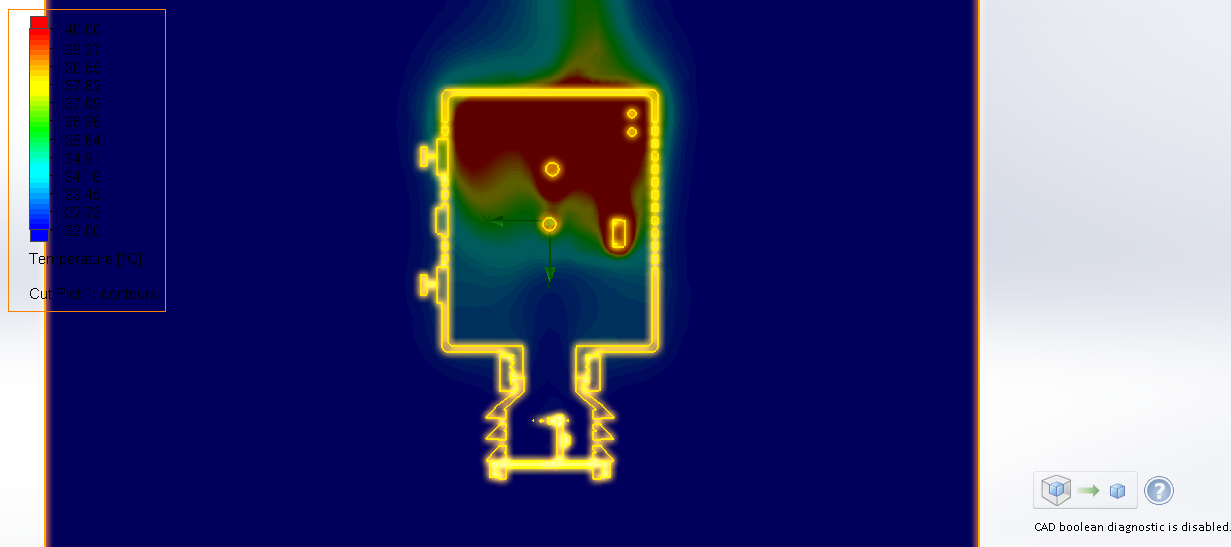
\includegraphics[width=\linewidth]{01 Temperature section front.png}
\caption{Temperature section (32--40\,\textdegree C scale). Hot air inside the box rises out of the top; the sensor holder below stays at room temperature.}
\end{figure}

\begin{figure}[H]
\centering
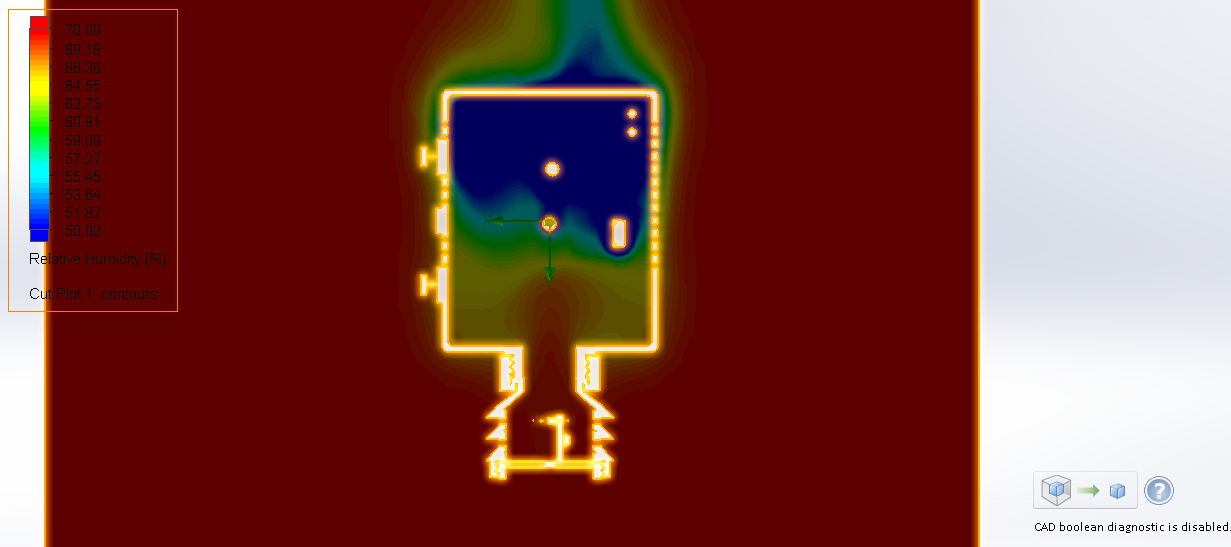
\includegraphics[width=\linewidth]{02 Relative humidity section front.png}
\caption{Relative humidity section (50--70\,\% scale). The sensor holder sees store-air humidity (red, about 70\,\%); only the warm box interior and the plume above are drier.}
\end{figure}

\begin{figure}[H]
\centering
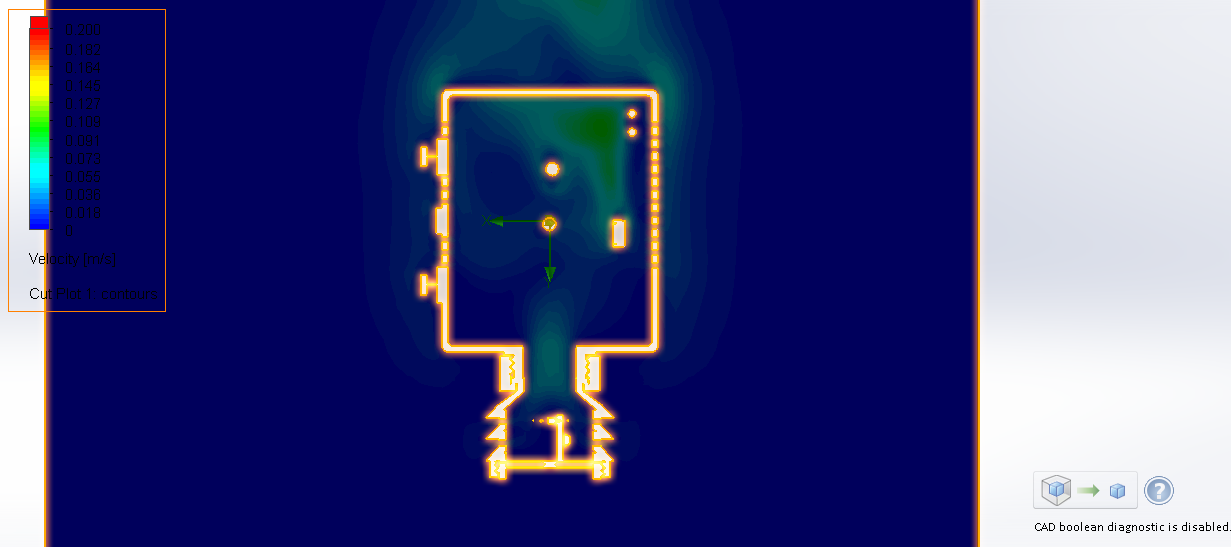
\includegraphics[width=\linewidth]{03 Air speed section front.png}
\caption{Air speed section (0--0.2\,m/s scale). The warm plume rises from the top of the box; air around the sensor holder is nearly still.}
\end{figure}

\begin{figure}[H]
\centering
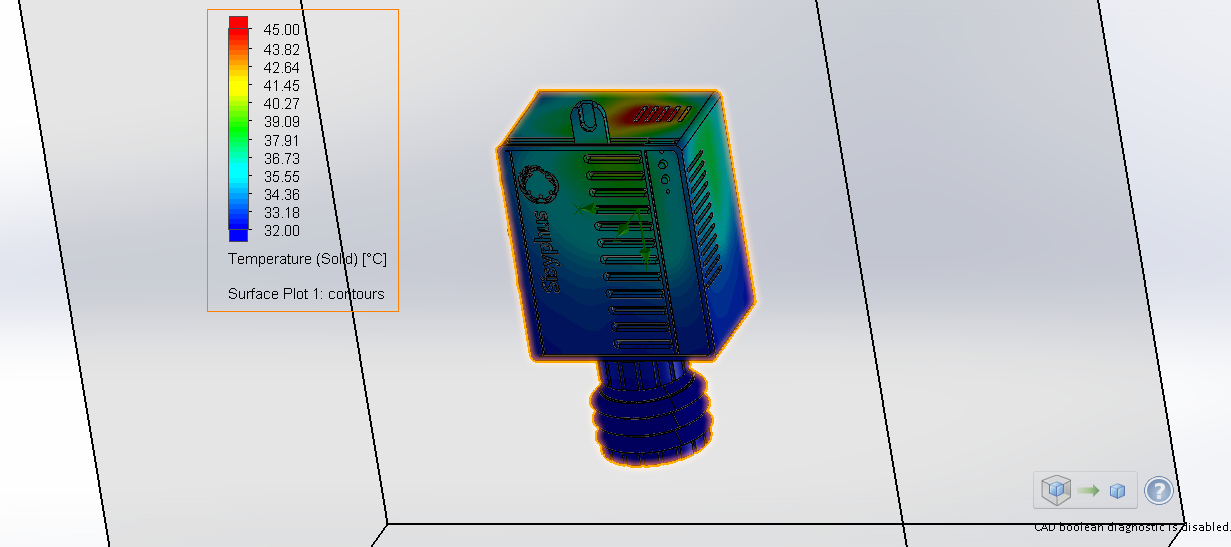
\includegraphics[width=\linewidth]{04 Surface temperature 3D.png}
\caption{Outer surface temperature (32--45\,\textdegree C scale). The top of the box around the upper vents and tab is warmest; the sensor holder stays at about 32\,\textdegree C.}
\end{figure}

%--------------------------------------------------------------------
\section{Design comparison: sensor above vs.\ below the box}
\begin{table}[H]
\centering
\begin{tabular}{l c c c c}
\toprule
Design & Sensor temp & Sensor RH & Error & Result \\
\midrule
Sensor \textbf{above} box (first run$^\dagger$)\SW & $\approx$49\,\textdegree C & 26--31\,\% & $\approx$+17\,\textdegree C / $\approx-$40\,\% RH\CALC & \bad \\
Sensor \textbf{below} box (final)\SW & 32.12\,\textdegree C & 68.9--69.7\,\% & +0.1\,\textdegree C / $-$1\,\% RH & \ok \\
\bottomrule
\end{tabular}
\end{table}
\small $^\dagger$The first run used PVC and no radiation, so it shows the trend, not an exact like-for-like comparison.\normalsize

%--------------------------------------------------------------------
\section{Design notes}
These are engineering judgements\EST\ based on the results.
\begin{itemize}
\item Keep the hanging orientation: tab up, sensor holder down.
\item Do not place anything sensitive directly above the device; the plume is 3--4\,\textdegree C warmer and up to 13\,\% RH drier.
\item Air inside the sensor holder moves slowly in still air (about 0.001--0.014\,m/s), so readings follow room changes over minutes, which is adequate for paddy storage.
\item PLA+ has a 4.6\,\textdegree C margin at 32\,\textdegree C with worst-case power. On hotter days (38--40\,\textdegree C) the margin is used up; PETG or ASA, or ESP deep sleep, is safer.
\end{itemize}

%--------------------------------------------------------------------
\section{Limitations}
\begin{itemize}
\item No store wall or paddy bags were modelled; the device hangs in open still air.
\item The sensor measures air near the device, not the air inside the paddy bags.
\item The 1.35\,W heat load is a worst-case estimate; with ESP deep sleep the real heat, and the sensor error, will be lower.
\item Hot spots inside the PCB (up to about 126\,\textdegree C) are not reliable because whole components were modelled as FR4; they do not affect the airflow or sensor results.
\item Probe values were transcribed from the SOLIDWORKS table on screen.
\end{itemize}

\end{document}
